\documentclass{beamer}
\usepackage[utf8]{inputenc}
\usepackage{amssymb}
\usepackage{amsmath}
\usepackage{dsfont}
\usepackage{stmaryrd}
\usepackage{graphicx}

\graphicspath{{./images/}}

\title{Optimisation stochastique, (RJ)MCMC et applications g\'eospatiales}
\author{}
\institute{IGN}
\date{2015}

\begin{document}
\frame{\titlepage}
 
\begin{frame}
\frametitle{Contexte}
\begin{itemize}
\item La recherche de l'IGN a souvent des probl\`emes d'optimisation (comme tout le monde)
\item D\'eveloppement d'outils \emph{sp\'ecifiques} (g\'en\'eralisation carto)
\item D\'eveloppement d'un biblioth\`eque plus \emph{g\'en\'erique}
\end{itemize}
\end{frame}

\begin{frame}
\frametitle{La \emph{libRJMCMC}}
Elle propose~:
\begin{itemize}
\item un \'echantillonneur RJMCMC
\item un recuit simul\'e (ou parallel tempering)
\item des exemples et des applications
\end{itemize}
Plusieurs impl\'ementations~:
\begin{itemize}
\item C++ (+ lien)
\item Java (+ lien)
\item Scala (+ lien)
\end{itemize}
Le tout sous licence libre.
\end{frame}

\section{Applications}

\begin{frame}
\frametitle{XXXX}
\emph{Le probl\`eme~:} 
\begin{itemize}
\item
\end{itemize}
\emph{Les concepts~:}

\begin{itemize}
\item MPP~:
\item A prioris~:
\item Noyaux~:
\item \'Energie~:
\end{itemize}
\end{frame}

\begin{frame}
\frametitle{XXXX}
\emph{R\'esultats:}
\end{frame}


\begin{frame}
\frametitle{Simplu3D}
\emph{Le probl\`eme~:}  Simulation des droits \`a batir
\begin{itemize}
\item Génération de configurations bâties pour évaluer l'influence des réglements des PLU
\end{itemize}
\emph{Les concepts~:}



\begin{columns}
\begin{column}{0.55\textwidth}
\begin{itemize}
\item MPP~:  $ \mathcal{C} =\cup_{n}( \mathcal{B})$  avec $\mathcal{B}  \subset  \mathds{R}^{6}$
\item Noyaux~: Naissance/mort, translation, rotation, changement de dimension (longueur, largeur ou hauteur)
\end{itemize}
\end{column}
\begin{column}{0.45\textwidth}
 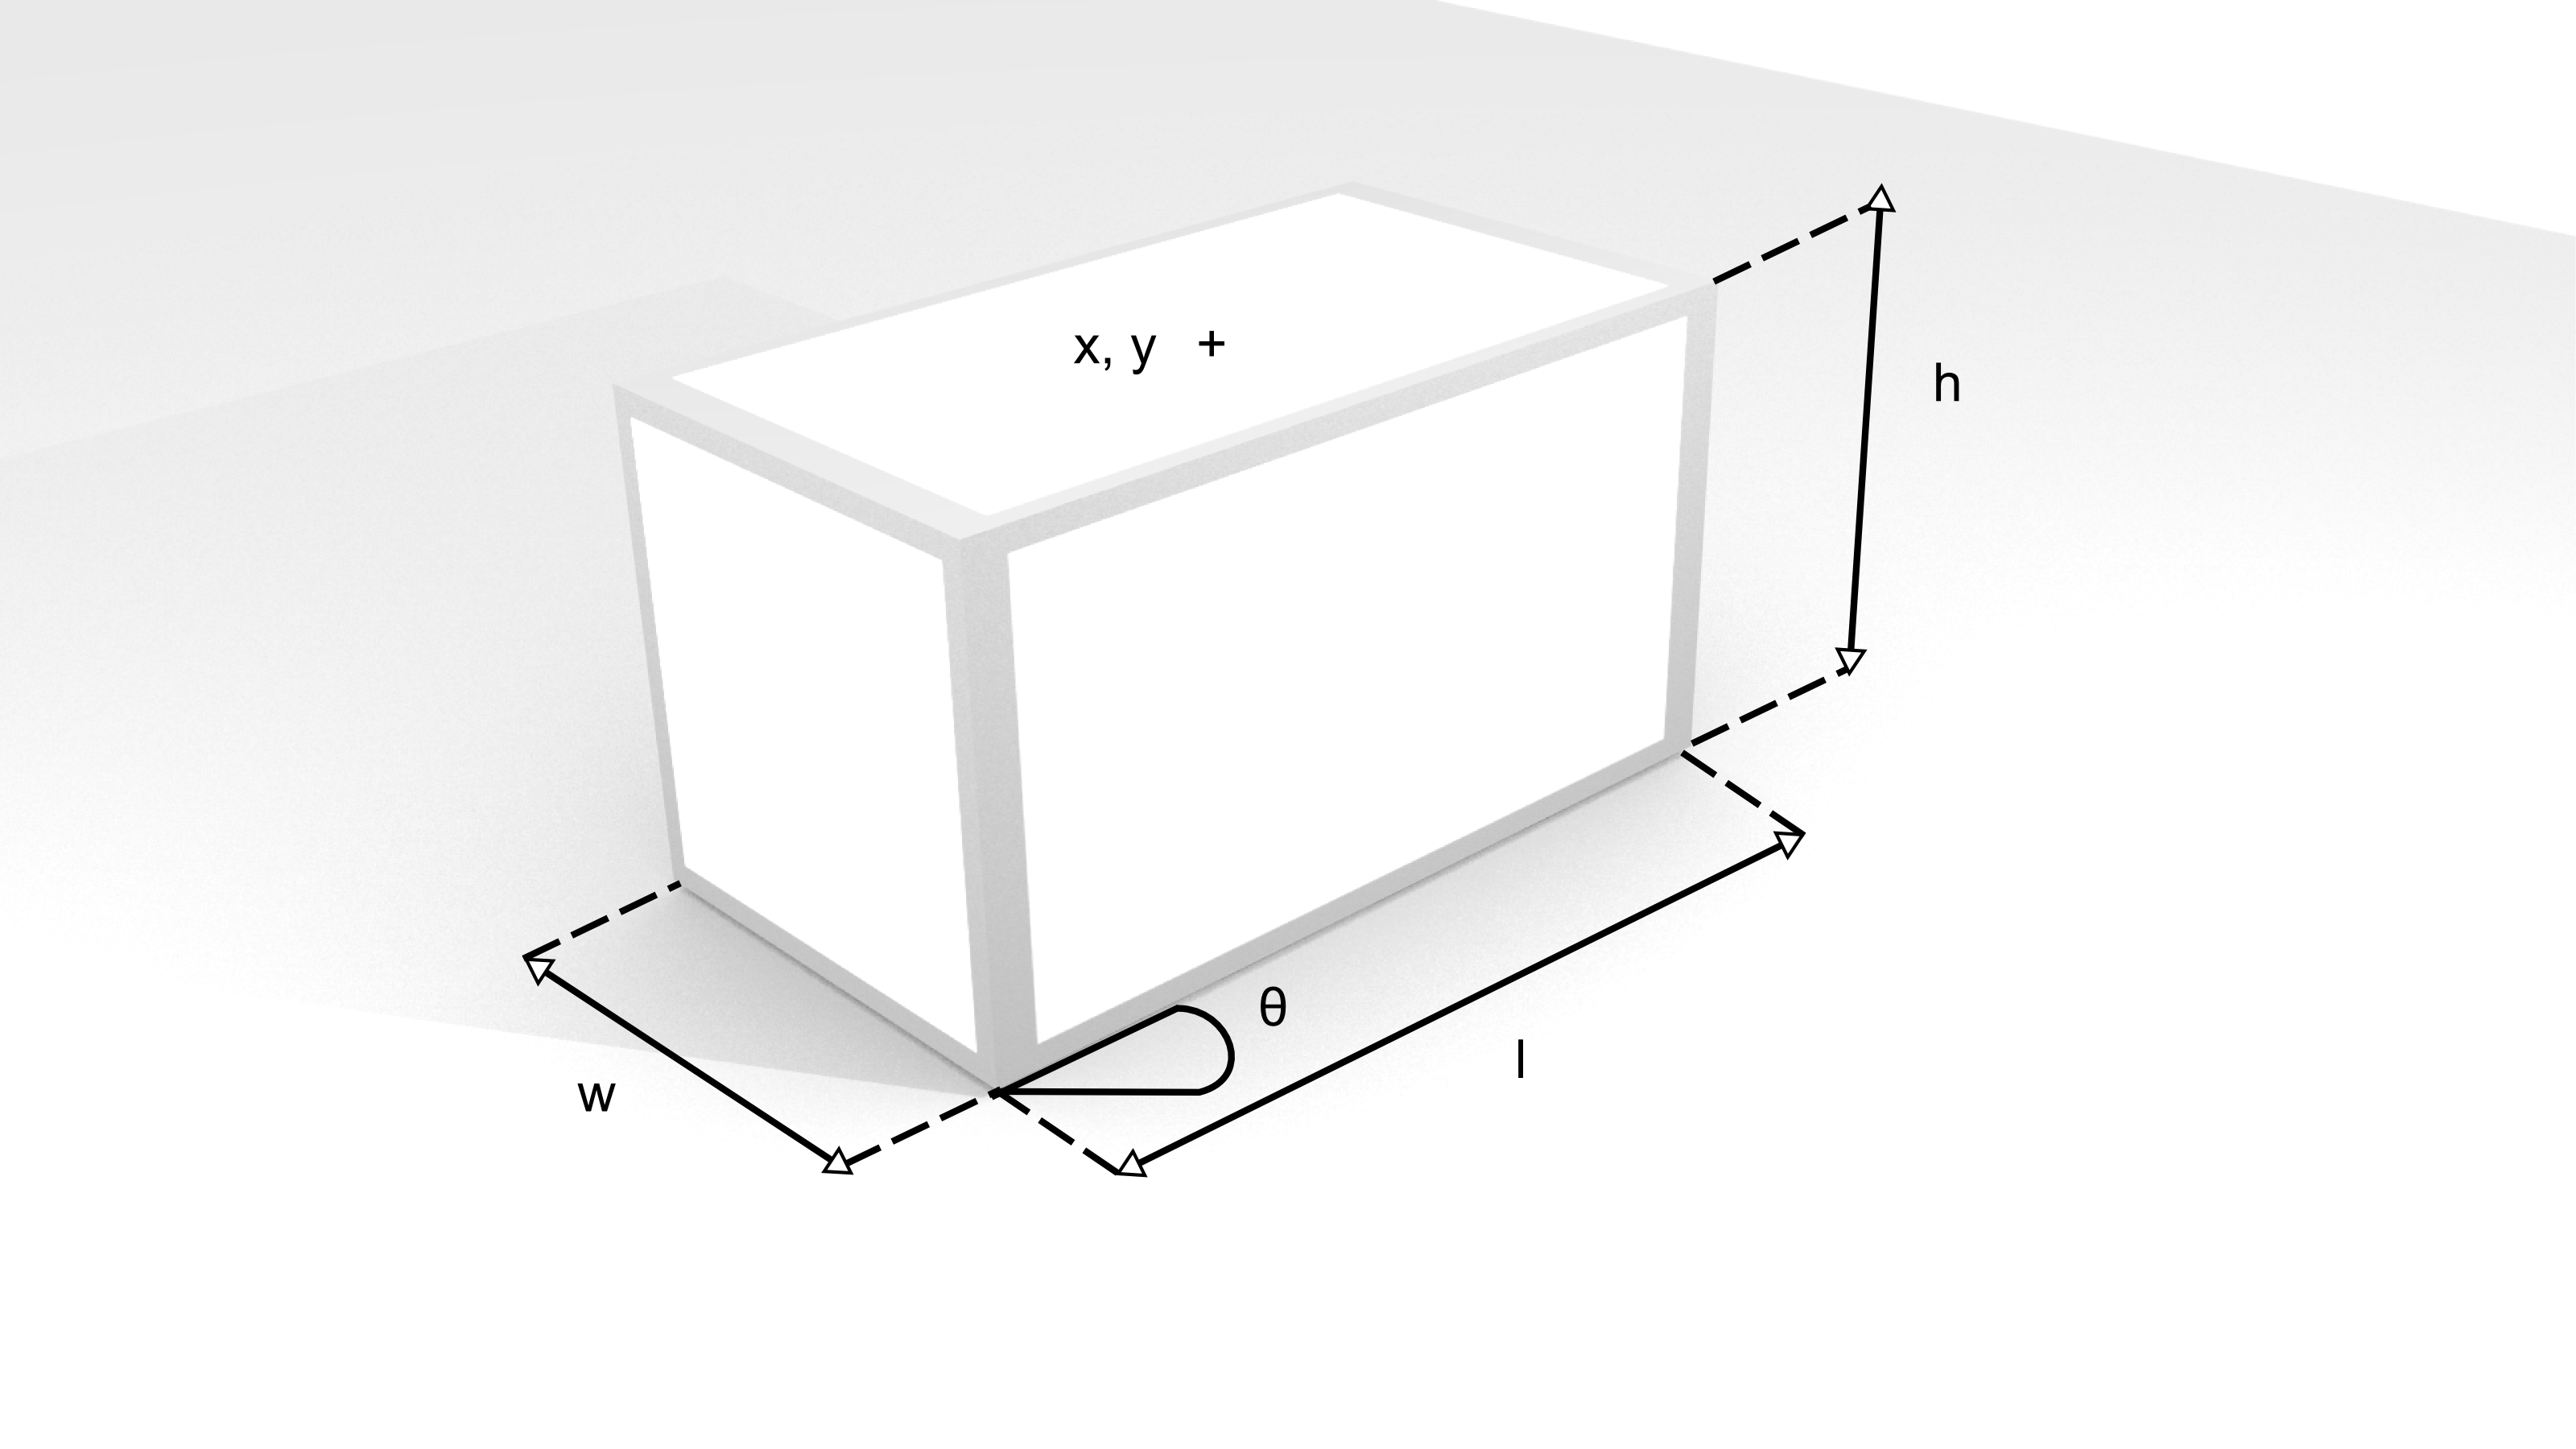
\includegraphics[width=\textwidth]{boiteFin.png}
\end{column}
\end{columns}
\begin{itemize}
\item Énergie~: $\mu = \mu_{unaire} + 2 \times \mu_{binaire}$
\begin{itemize}
\item $\tilde \mu_{unaire}(b \in \mathcal{B})=\alpha_{0} - volume(b)$ avec $\alpha_{0} \in \Re^{+*}$ ;
\item $\tilde \mu_{binaire}(b \in \mathcal{B}, b' \in \mathcal{B})) = volume(b \cap b')$.
\end{itemize}
\item Contraintes~:  $ \mathcal{S} = \mathcal{PLU} \cap  \mathcal{C}   $
\end{itemize}


\end{frame}

\begin{frame}
\frametitle{Simplu3D}
\emph{R\'esultats:}
 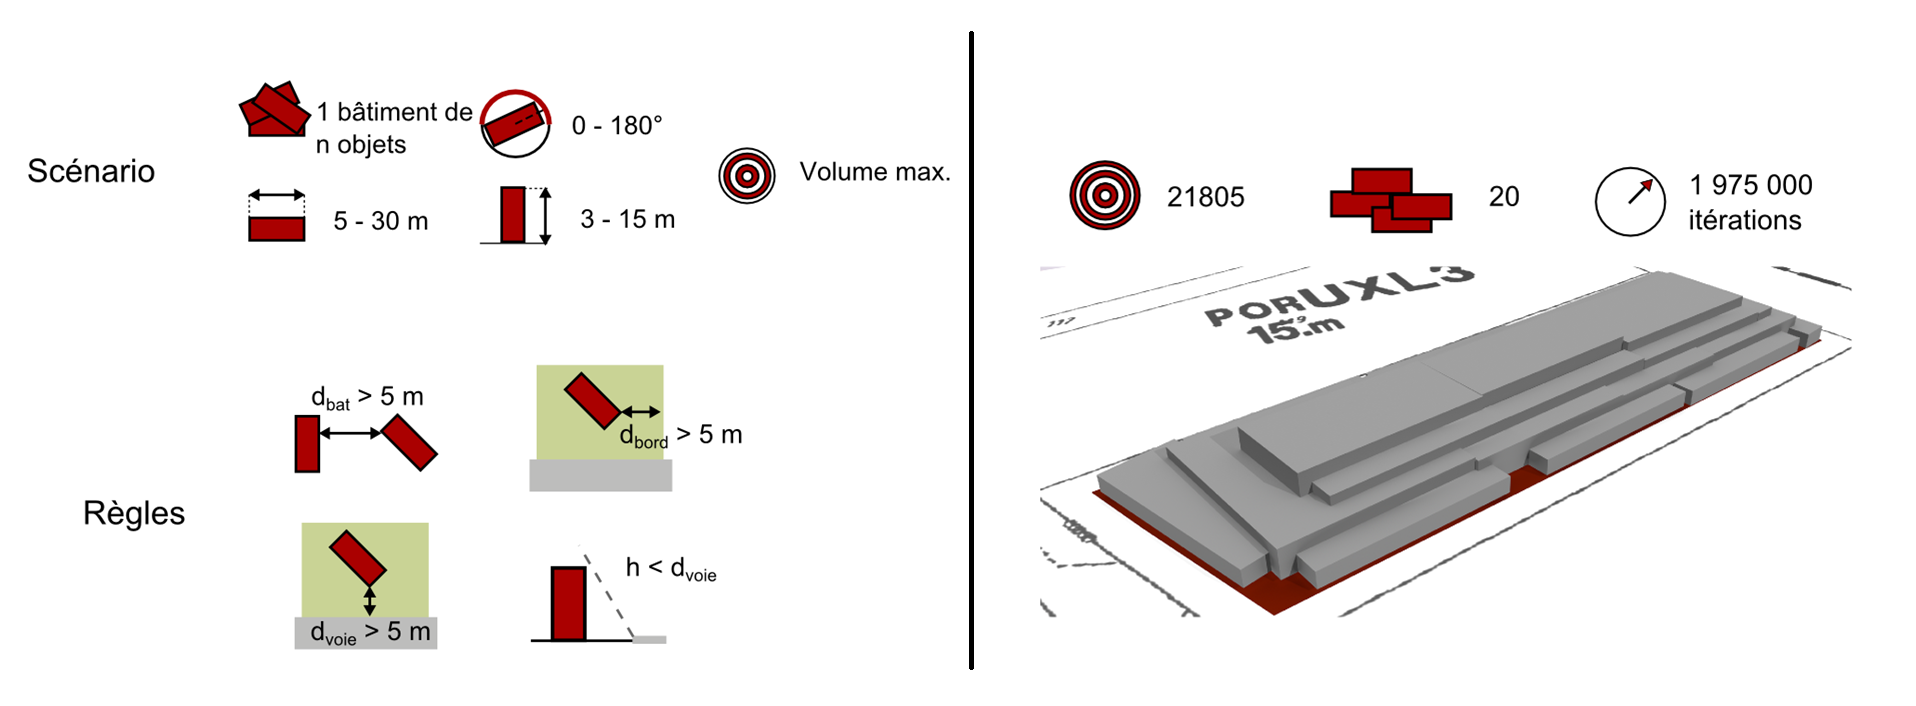
\includegraphics[width=\textwidth]{simplu3D1.png}
\end{frame}

\begin{frame}
\frametitle{Simplu3D}
\emph{R\'esultats:}
 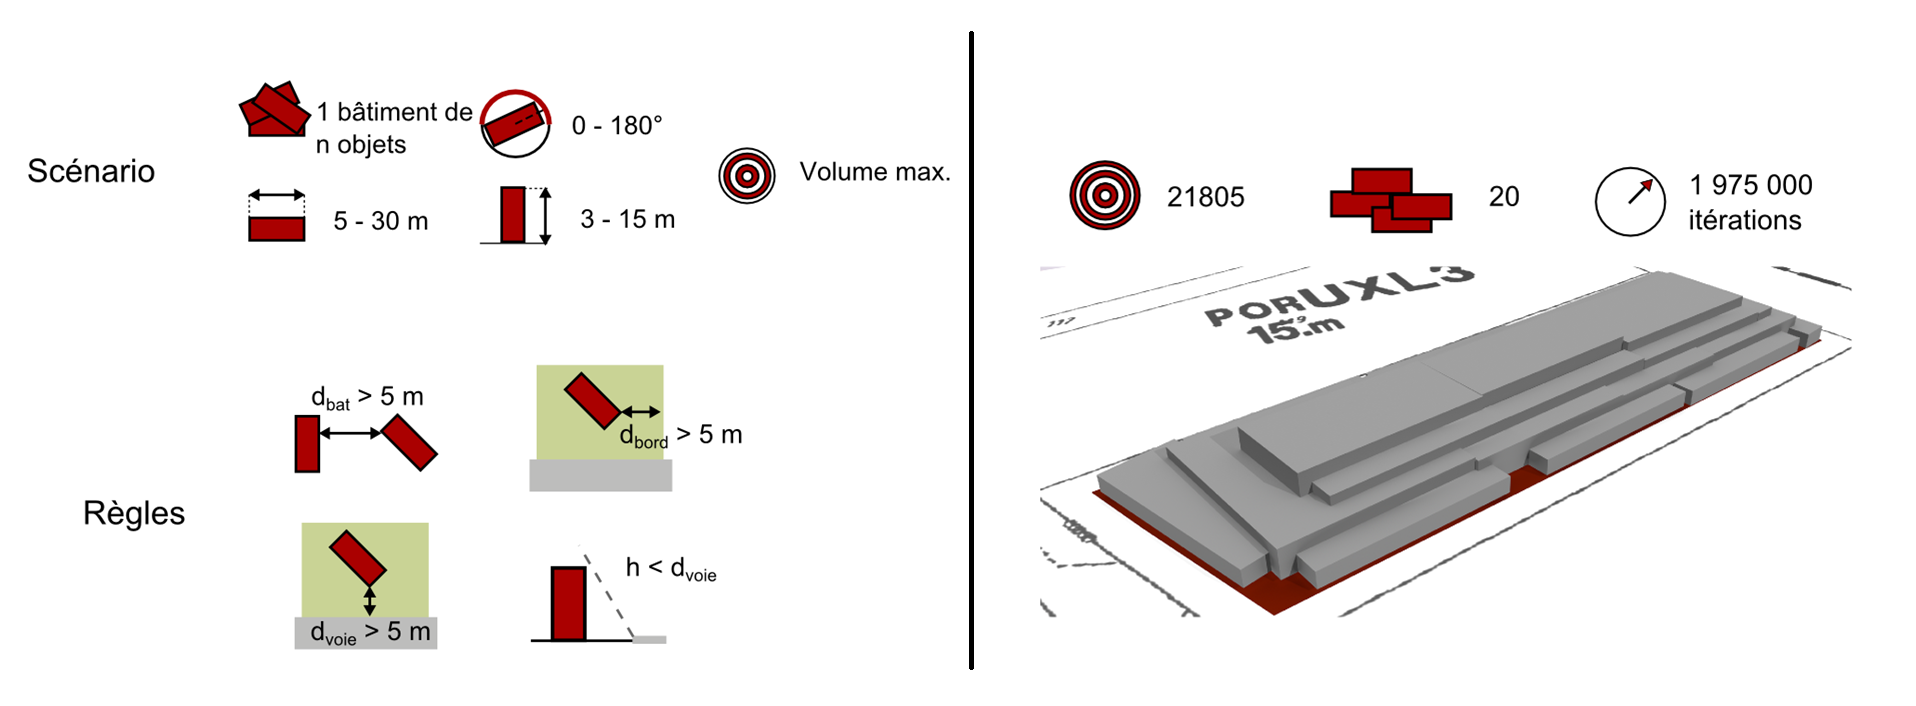
\includegraphics[width=\textwidth]{simplu3D1.png}
\end{frame}

\begin{frame}
\frametitle{Simplu3D}
\emph{R\'esultats:}
 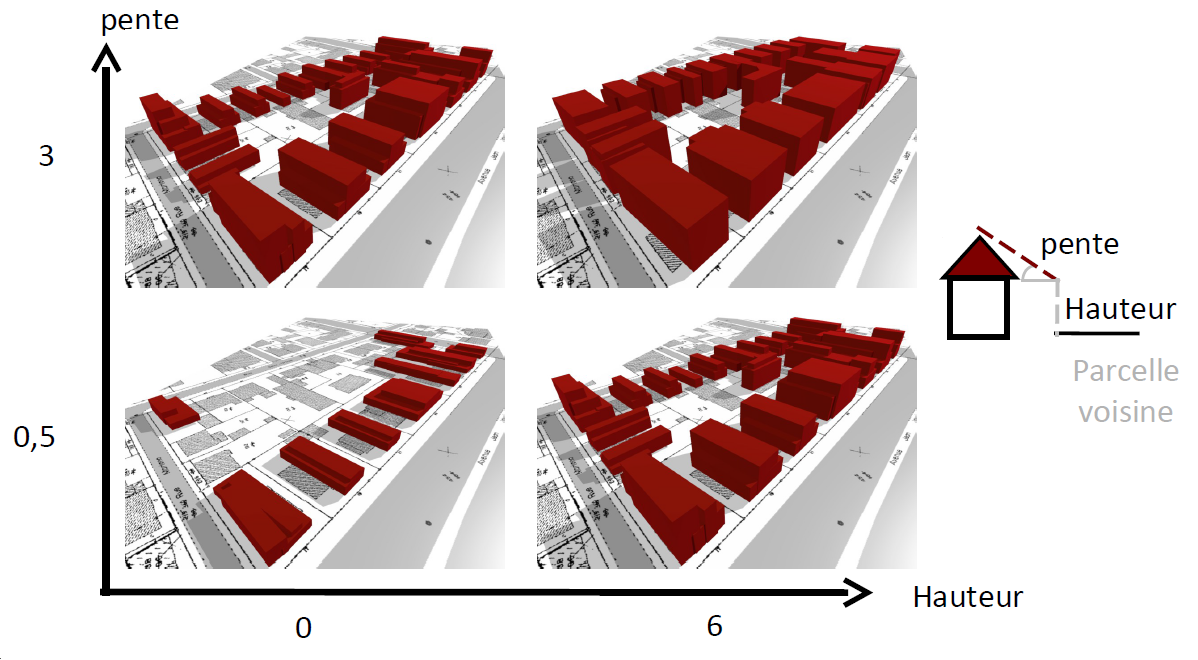
\includegraphics[width=\textwidth]{simplu3D2.png}
\end{frame}

\end{document}
